% META: {"id": "1NSI-ADGK-CO-010", "chapitre": "1NSI-ALGO-PARCOURS-TRIS", "type_objet": "correction", "exercice_ref": "1NSI-ADGK-EX-010", "capacites_codes": ["C2"], "sources_inspiration": [], "status": "approved", "capacites": ["1NSI-ALGO-PARCOURS-TRIS-C2"], "parcours": 2, "duree_min": 2, "fichier_exercice": "chapitres/1NSI-ALGO-PARCOURS-TRIS/exercices/1NSI-ADGK-EX-010.tex", "mode_creation": "ex_nihilo"}
% BEGIN-VERIFY
% from sympy import *
% x = symbols('x')
% f = x**3 - 3*x**2 + 2
% fp = diff(f, x)
% assert expand(fp) == 3*x**2 - 6*x
% assert solve(fp, x) == [0, 2]
% assert f.subs(x, 0) == 2
% assert f.subs(x, 2) == -2
% assert limit(f, x, -oo) == -oo
% assert limit(f, x, oo) == oo
% END-VERIFY
\begin{corrige}{1NSI-ADGK-EX-010}

\commentaireMarge{Dériver, factoriser, étudier le signe.}

$f'(x) = 3x^2 - 6x = 3x(x - 2)$.

\begin{center}
\begin{tikzpicture}

ode {$f'(x)$ : $+$ sur $\left]-\infty, 0\right[$, $-$ sur $\left]0, 2\right[$, $+$ sur $\left]2,+\infty\right[$.};
\end{tikzpicture}
\end{center}

$f(0) = 2$ (maximum local), $f(2) = -2$ (minimum local).

$f$ est croissante sur $\left]-\infty, 0\right]$, decroissante sur $[0, 2]$, croissante sur $[2, +\infty[$.

\end{corrige}
